\documentclass[11pt]{exam}
\usepackage{listings}
\usepackage{pdfsync}

\newif\ifpdf
\ifx\pdfoutput\undefined
\pdffalse % we are not running PDFLaTeX
\else
\pdfoutput=1 % we are running PDFLaTeX
\pdftrue
\fi

\ifpdf
\usepackage{subfigure}
\usepackage[pdftex]{graphicx}
\else
\usepackage{graphicx}
\fi

\firstpageheader{\bf\Large CS 151}{\bf\Large Exam-2}{\bf\Large
  April 9, 2007}
\runningheader{CS 151}{}{Exam-2}
\addpoints

\begin{document}
\begin{center} 
  \fbox{\fbox{\parbox{5.5in}{\centering This Exam is being given under
        the guidelines of the \textbf{Honor Code}. You are expected to
        respect those guidelines and to report those who do not.
        Answer the questions in the spaces provided. If you run out of
        room for an answer, continue on the back of the page.  There are
      \numquestions\  questions for a total of  \numpoints\ points.}}}
\end{center} 
\lstset{language=Python,numbers=left}

\vspace{0.1in} 
\hbox to \textwidth{Name:\enspace\hrulefill} 


\begin{questions}

\question[5] The following diagram contains plots the running times of algorithms that are:
\begin{itemize}
\item $O(N)$
\item $O(log_2 N)$
\item $O(1)$
\item $O(N^3)$
\item $O(N^2)$
\end{itemize}
Label each line on the graph with the appropriate big $O$ function.

\begin{figure}[h!b]
	\begin{center}
		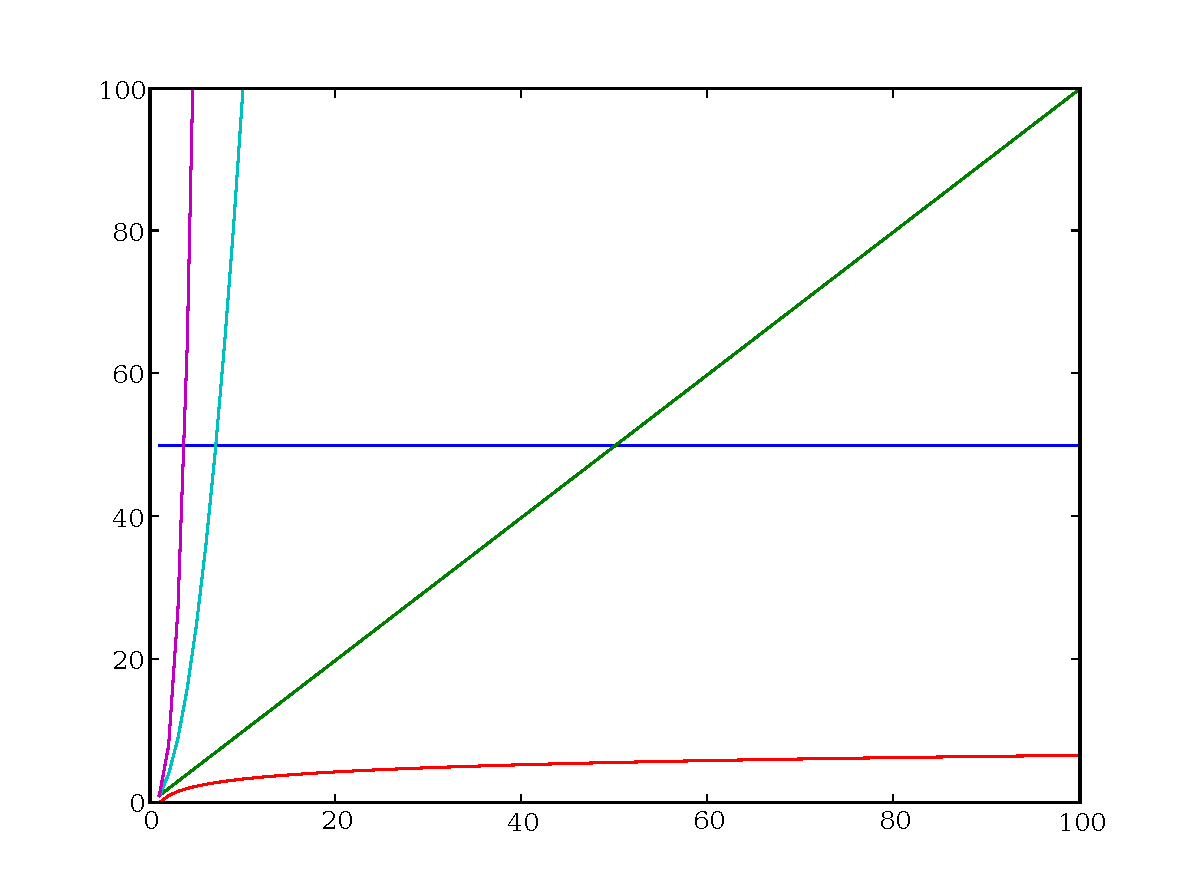
\includegraphics[scale=.75]{bigo}
	\end{center}
	\label{fig:bigo}
\end{figure}


% remove duplicates from a list
\newpage
\question[10] 
Write an  $O(n)$, algorithm that will remove all duplicates letters from a string.  You can use any Python functions or data types you want, but you must explain the running time of anything you use.
\vspace{4.5in}


%\question[10] Given the following list \lstinline{L = [90, 1, 3, 8, 56, 21, 5, 13, 1, 146, 2, 34]}.  Show the contents of \lstinline{L} after the first two passes of Selection sort.

\newpage
\question[10] Given the following list of numbers \texttt{a = [ 90, 1, 3, 8, 56, 21, 5, 13, 1, 146, 2, 34]}.  Show the contents of $a$ during \texttt{shell} sort, after a gap size of 5.
\vspace{4.5in}


\question[10] Given the following list 
\lstinline{L = [11, 3, 23, 17, 9, 21, 7, 5, 1, 19, 13, 15]}.  Show the contents of \lstinline{L} after one partition by \texttt{Quicksort}.  You should use the median of three pivot selection method.
\vspace{4.5in}


\question[5]  What is the Big-O running time for the following code fragment:
\begin{lstlisting}[language=python]
sum = 0
i = 1
while i < n:
    sum = sum + 1
    i = i * 2
\end{lstlisting}
\vspace{.5in}

\question[5]  What is the Big-O running time for the following code fragment:
\begin{lstlisting}[language=python]
sum = 0
for i in range(n):
    sum = sum + 1
for j in range(n):
    for k in range(n+1):
        for l in range(n+2)
            sum = sum + 1
\end{lstlisting}
\vspace{.5in}

\question[10] Write a recursive algorithm to compute $x^n$, given two numbers $x > 0$, and $n > 0$.
\vspace{4.5in}

\question[10] Given the following list \lstinline{L = [1, 3, 5, 7, 9, 11, 13, 17, 19, 23]} write down each comparison that the \texttt{binarySearch} algorithm would do when searching for the key 7.
\vspace{4in}

\question[10] Given the following set of keys show the resulting hash table assuming that you are using linear probing.  Insert them in order from left to right.  The table holds exactly 11 keys.  You do not need to worry about growing the table.  Use a simple \lstinline{x % 11} function on the keys.

\begin{table}[h!]
	\begin{center}
	\begin{tabular}{|c|c|c|c|c|c|c|c|c|}
    113 & 117 & 95 & 106 & 114 & 108 & 116 & 105 & 99 \\
     \end{tabular}
	\end{center}
	\label{htab}
\end{table}
\vspace{3in}


\end{questions}

\end{document}

